% \chapter{Лекция}
% \label{ch:intro}

% \section*{Что такое SDR?}

% \textbf{Software-Defined Radio (SDR)} - радиосистема, в которой 
% традиционно аппаратные компоненты (фильтры, модуляторы, демодуляторы, детекторы, кодеры и т.п.) 
% реализованы на программном уровне, с использованием универсального оборудования и цифровой обработки сигналов.

% \section*{Базовая архитектура системы радиосвязи}

% Картинка1 \\

% \section*{Описание компонентов архитектуры}

% Базовая архитектура состоит из \textbf{передатчика (TX)} и \textbf{приемника (RX)}. Между ними находится \textbf{радиоканал - среда}, в которой распространяется сигнал. У \textbf{TX} и \textbf{RX} есть \textbf{антенна - устройство}, которое излучает или принимает электромагнитные волны, и преобразует их в электрический ток и обратно, в самом простом случае это просто кусок проволоки. Также и у \textbf{TX} и у \textbf{RX} есть \textbf{усилитель}, который усиливает отправляемый/принимаемый сигнал.

% \section*{Описание процесса обмена данными}

% На стороне \textbf{TX} формируется \textbf{сообщение}, которое необходимо передать. Это сообщение поступает в передатчик в виде набора \textbf{нулей и единиц}. \textbf{TX} преобразует нули и единицы определенным образом в электрические колебания, которые через \textbf{антенну} излучаются в виде электромагнитных колебаний в радиоканал.\\
% В этом же радиоканале находится \textbf{приемник}, \textbf{антенна} которого принимает эти электромагнитные колебания и преобразует в электрический ток. После этого электрические колебания определенным образом преобразуется в набор нулей и единиц (сообщение, которое отправлял \textbf{TX}). Стоит отметить, что \textbf{прием сообщения} намного сложнее, чем отправка. Это связано с изменениями, которым подвергается сигнал во время прохождения через \textbf{радиоканал}. Сигнал изменяется случайным образом, поэтому точно сказать, как изменится сигнал, мы не можем, мы можем это только предположить с какой-то точностью. Эта проблема решается путем добавления в исходный сигнал \textbf{избыточности}, которая позволяет с более высокой точностью принять сигнал на стороне приемника. Такой избыточностью может быть \textbf{контрольная сумма - число}, которое вычисляется по определенному алгоритму, который учитывает позицию бита и его значение, т.е если хоть в какой нибудь позиции изменится значение бита, то \textbf{контрольная сумма} будет уже другой, что сигнализирует об искажении сигнала.

% \section*{Внутренняя архитектура TX}

% картинка2 \\

% \section*{Coder}

% Устройство или программный модуль, предназначенный для \textbf{преобразования исходных данных в кодированное представление}. 

% \medskip

% Основные функции кодера:
% \begin{itemize}
%     \item \textbf{Преобразование данных} - перевод информации (например, текста, аудио, видео, сигналов) в определённый формат или код.
%     \item \textbf{Сжатие} - уменьшение объёма данных за счёт использования специальных алгоритмов кодирования.
%     \item \textbf{Обеспечение помехоустойчивости} - добавление избыточности в данные для защиты от ошибок при передаче по каналу связи.
%     \item \textbf{Совместимость} - приведение данных к стандартному виду, который может быть правильно обработан устройством-приёмником.
% \end{itemize}

% В нашем самом простом случае кодер будет выполнять единсвтенную задачу - формировать из потока бит блоки (допустим по 8 бит) и
% направлять их в Mapper.

% \section*{Mapper}

% Устройство или программный модуль, выполняющий \textbf{отображение исходных данных на множество символов или сигналов} в соответствии с выбранной схемой модуляции или кодирования. 

% \medskip

% Основные функции маппера:
% \begin{itemize}
%     \item \textbf{Отображение битов на символы} - преобразование двоичной последовательности в набор сигналов (например, QPSK, QAM).
%     \item \textbf{Подготовка к модуляции} - формирование последовательности комплексных чисел, которые могут быть использованы модулятором.
%     \item \textbf{Оптимизация передачи} - использование схем отображения, минимизирующих вероятность ошибки при передаче (например, Gray-код).
%     \item \textbf{Гибкость} - возможность выбора различных карт маппинга в зависимости от условий канала и требований к системе.
% \end{itemize}

% В нашем самом простом случае mapper будет выполнять единсвтенную задачу - отображать исходные биты на множество символов. \\

% Символ - элемент сиганльного множества. \\

% Сигнальное мн-во - набор состояний радиосигнала. \\

% Иными словами: mapper берет блок битов (у нас это 8 бит) и сопоставляет его сигналу с определенными характеристиками, для 
% этого в mapper хранится "таблица" с комбинациями битов и соответсвующие им символы. Если в блоке
% 8 бит, то всего должно быть 256 символов (на каждую возможную комбинацию). \\

% Пример таблицы \\

% Также для визуализации данного процесса используется созвездие символов \\

% \textbf{Созвездие символов} - это \textbf{графическое представление множества возможных символов модуляции} в комплексной плоскости.  
% Каждый символ соответствует определённой комбинации параметров сигнала (амплитуды и фазы), и изображается в виде точки на диаграмме.  

% \begin{figure}[H]
%     \centering
%     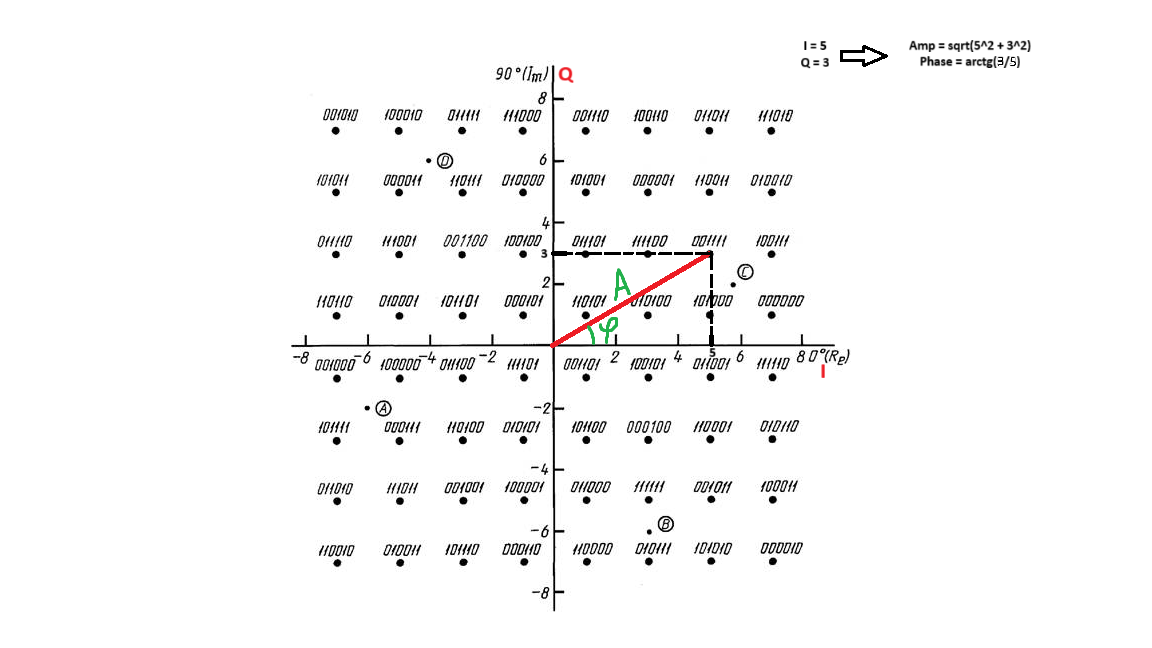
\includegraphics[width=1.0\textwidth]{QAM64.png}
%     \caption{Пример созвездия символов}
% \end{figure}

% Каждой точке соответствуют координаты (I, Q), где I - действительная составляющая, Q - мнимая. Зная координаты, можем вычислить
% длину радиус-вектора до этой точки, это будет амплитудой этого сигнала, угол между действительной осью и радиус-вектором - фаза
% сигнала.

% От mapper идет 2 выхода, один для I составляющей, другой для Q составляющей, которые поступают на вход формирующего фильтра.

% \subsection*{Немного про I/Q семплы}

% Запишем сигнал и распишем с помощью формулы аргументов косинусов. \\

% $$S_c(t) = A(t)cos(2\pi f_ct + \phi(t)) = A(t)cos\phi(t)*cos(2\pi f_ct) - A(t)sin\phi(t)*sin(2\pi f_ct)$$

% Здесь $A(t)cos\phi(t)$ - синфазная часть сигнала (I), а $A(t)sin\phi(t)$ - квадратурная часть (Q). \\

% Таким образом, зная I и Q можно создать сигнал, и mapper как раз нам эти I/Q и дает. \\

% Все это называется QAM-модуляцией (Quadrature Amplitude Modulation) - технология передачи цифрового информационного потока в виде аналогового
% сигнала. Это достигается путем разделения несущей волны на две несущие одинаковой
% частоты сдвинутые относительно друг-друга на 90 градусов.

% \section*{Формирующий фильтр}


% Устройство или программный модуль в системе передачи данных, предназначенный для преобразования последовательности символов в непрерывный сигнал с заданной временной формой, оптимальной для передачи по каналу связи.  

% \textbf{Математическое описание:}
% \[
% s(t) = \sum_{k=-\infty}^{\infty} a_k \, h(t - kT)
% \]
% где:
% \begin{itemize}
%     \item $s(t)$ --- сигнал на выходе формирующего фильтра,
%     \item $a_k$ --- последовательность передаваемых символов,
%     \item $h(t)$ --- импульсная характеристика фильтра,
%     \item $T$ --- период передачи символа.
% \end{itemize}

% \textbf{Функции формирующего фильтра:}
% \begin{enumerate}
%     \item Формирование импульсной формы сигнала для минимизации межсимвольной интерференции (ISI).
%     \item Ограничение спектра передаваемого сигнала для уменьшения влияния шумов и помех.
%     \item Обеспечение соответствия сигнала требованиям канала связи (например, полосе пропускания).
%     \item Подготовка сигнала к последующей модуляции и передаче.
% \end{enumerate}

% На этом этапе необходимо превратить символы (из I и Q) в длительные (передаваемые) символы (символы, растянутые по по времени с длиной $T_s$)

% \begin{figure}[H]
%     \centering
%     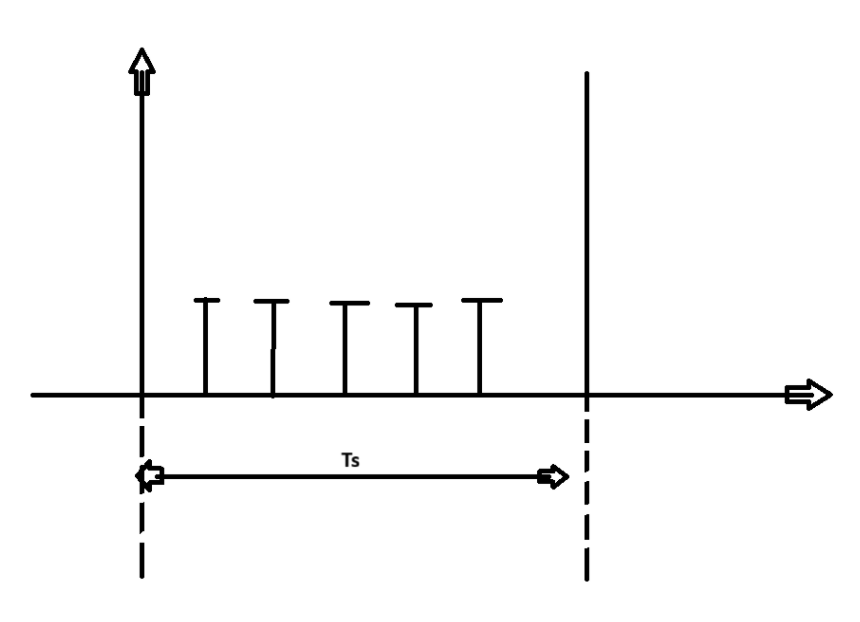
\includegraphics[width=1.0\textwidth]{pulse.png}
%     \caption{Пример длительного символа}
% \end{figure}

% До этого момента все выполнялось программно, т.е это зона ответственности программиста, всё, что будет дальше - работа самой SDR. \\

% Далее происходит двухканальная модуляция, где и происходит генерация непрерывного сигнала. Математически этот процесс можно записать
% следующим образом:

% $$s(t) = I(t)\cos(2\pi f_c t) - Q(t)\sin(2\pi f_c t)$$

% $f_c$ здесь - несущая частота (высокочастотное колебание).

% \endinput